\section{Результаты}
\subsection{Выбор параметров метода отжига}
Важнейшим фактором в сходимости метода отжига является выбор его параметров. Часть параметров, такие как начальная и конечная температура, а также кол-во испытаний на один температурный уровень, мы будем подбирать для каждой функции отдельно. Здесь же зафиксируем правило перехода $\mathcal{S}(\mathbf{Y})$, а также параметр $\alpha$ для уменьшения температуры.\\
В представленном выше алгоритме \eqref{SimAnnAlgo} при приближении к минимуму мы постоянно будет уменьшать радиус ведущего бруса. Пусть ведущий брус всегда храниться последним в списке, тогда чтобы не обращаться к брусам из начала списка спустя множество итераций, определим правило перехода как
\begin{equation}
    \mathcal{S}(\mathbf{Y})=\frac{|L\cdot N(0,\sigma^2)|}{3\sigma},\quad \sigma=||\mathrm{wid}(\mathbf{Y})||
\end{equation}
где $L$ - текущий размер рабочего списка, а $N(0,\sigma^2)$ - случайная величина, имеющая нормальное распределение с центром в нуле.
Таким образом $\mathcal{S}(\mathbf{Y})$ будет отвечать у нас за смещение от ведущего бруса в рабочем в списке. Можно заметить, что таким образом мы можем выйти за границы рабочего списка, поэтому определим индекс нового бруса $\mathbf{Z}$ как
\begin{equation}
    I_{\mathbf{Z}}=\max(1, L - \mathcal{S}(\mathbf{Y}))
\end{equation}
Предполагается, что индексация рабочего списка, начинается с 1.\\\\
Эмпирическим путём было выявлено, что оптимальным значением коэффициента $\alpha$ является $\alpha=0.8$, поэтому будем использовать его для всех функций.
\subsection{Функция МакКормика}
Для функции МакКормика положим $T_0=10^{-2}, T_{\mathrm{fin}}=10^{-16}$ и $N_T=25$.
\begin{figure}[H]
\centering
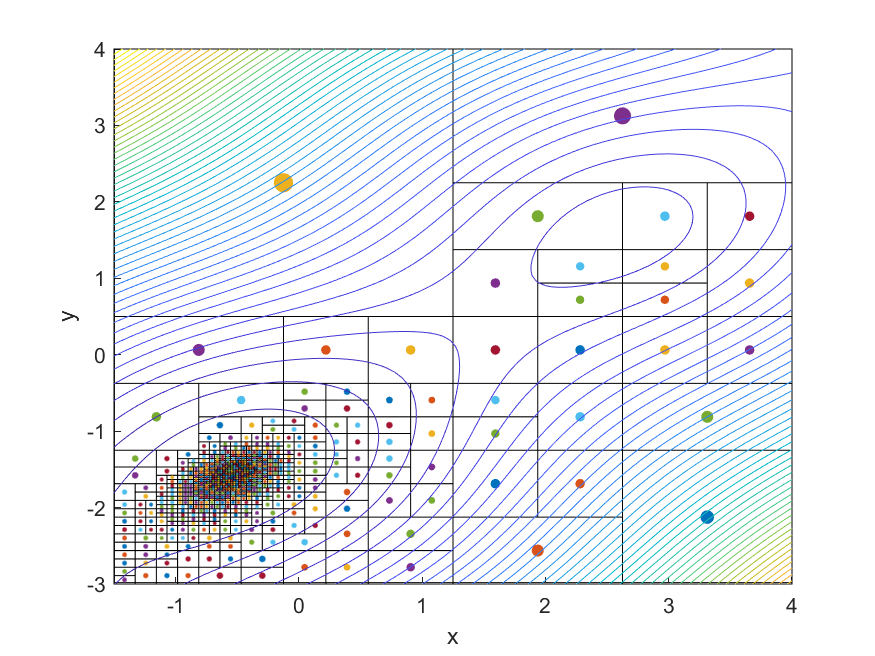
\includegraphics[width=0.9\textwidth]{Graphics/TrivialDivide_McCormick_algo.png}
\caption{Работа простейшего алгоритма дробления для функции МакКормика \eqref{McCormick}} 
\end{figure}
\begin{figure}[H]
\centering
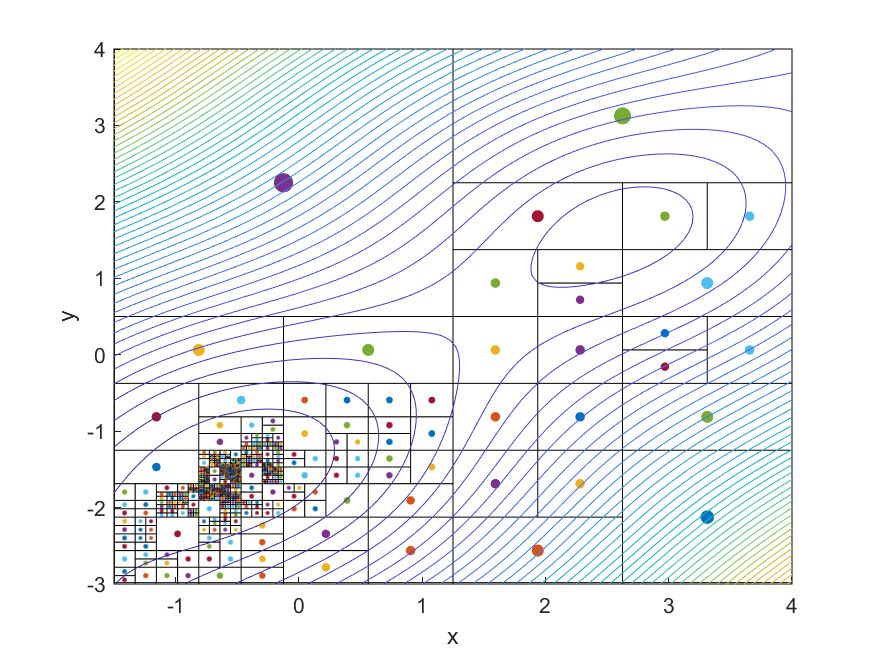
\includegraphics[width=0.9\textwidth]{Graphics/SimAnnealing_McCormick_algo.png}
\caption{Работа метода отжига для функции МакКормика \eqref{McCormick}} 
\end{figure}
\begin{figure}[H]
\centering
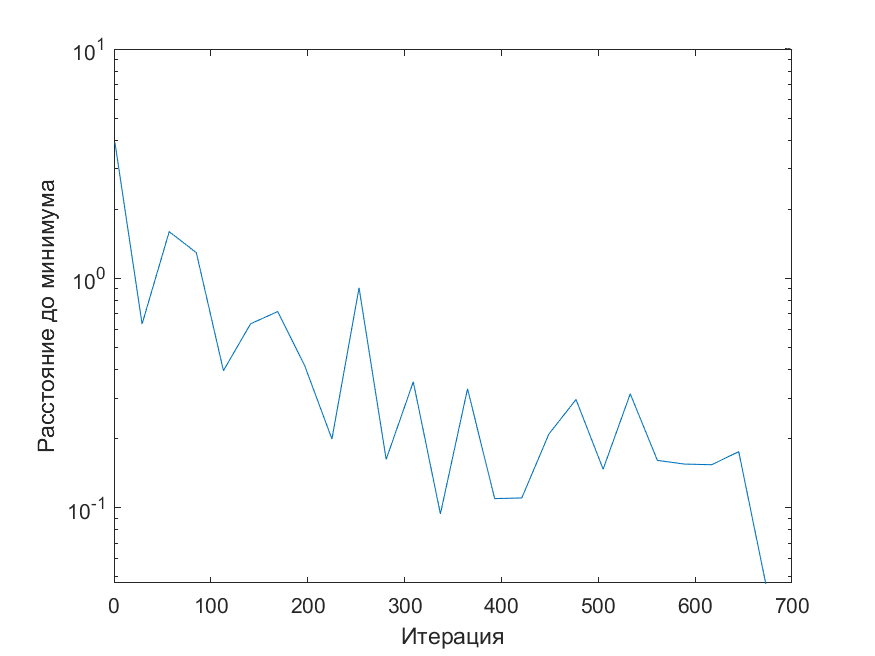
\includegraphics[width=0.9\textwidth]{Graphics/TrivialDivide_McCormick_dist_to_min.png}
\caption{Расстояния до минимума простейшего алгоритма дробления\\ для функции МакКормика \eqref{McCormick}} 
\end{figure}
\begin{figure}[H]
\centering
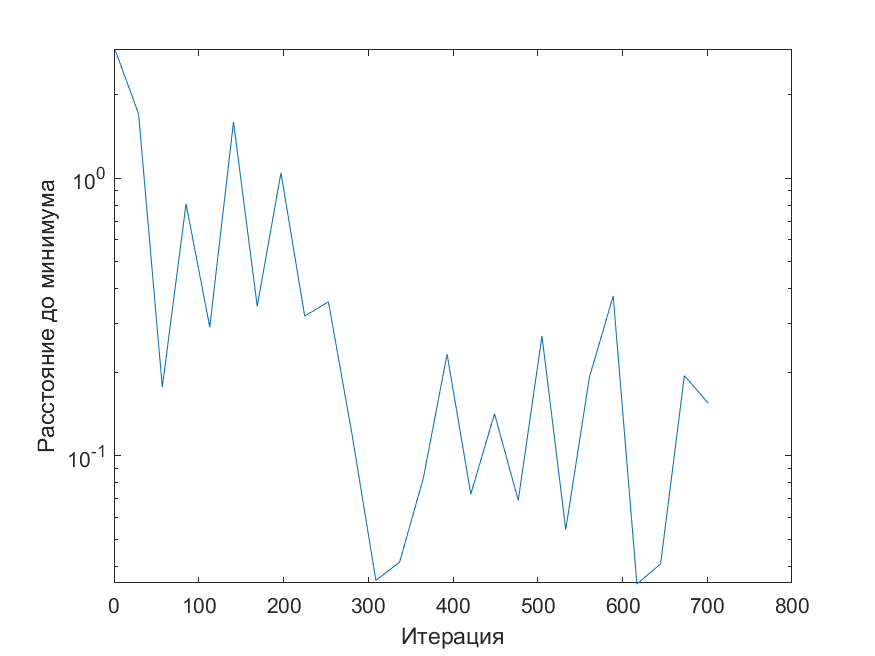
\includegraphics[width=0.9\textwidth]{Graphics/SimAnnealing_McCormick_dist_to_min.png}
\caption{Расстояния до минимума метода отжига для функции МакКормика \eqref{McCormick}} 
\end{figure}
\subsection{Функция Изома}
Для функции Изома положим $T_0=10^{-3}, T_{\mathrm{fin}}=10^{-10}$ и $N_T=10$.
\begin{figure}[H]
\centering
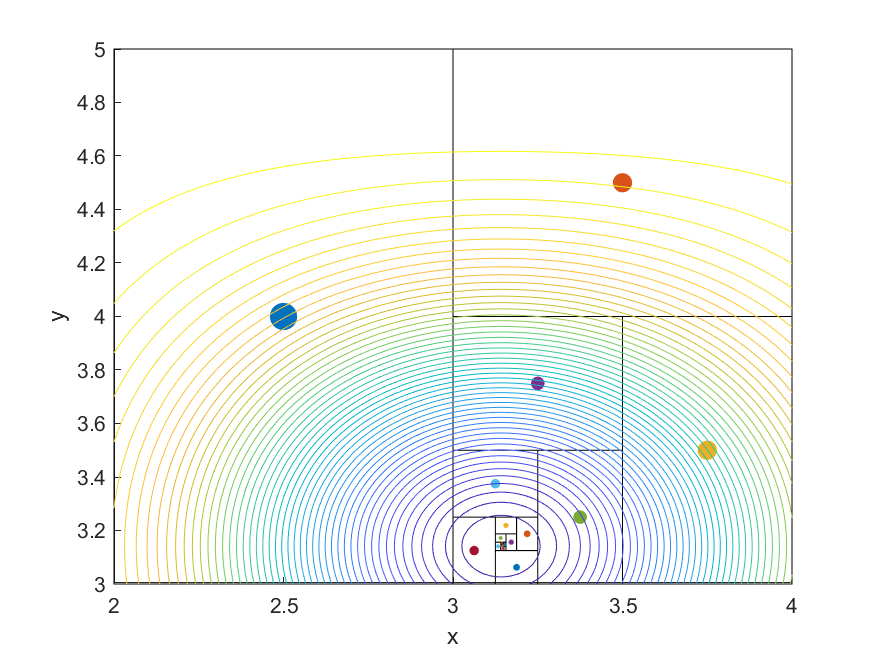
\includegraphics[width=0.9\textwidth]{Graphics/TrivialDivide_Easom_algo.png}
\caption{Работа простейшего алгоритма дробления для функции Изома \eqref{Easom}} 
\end{figure}
\begin{figure}[H]
\centering
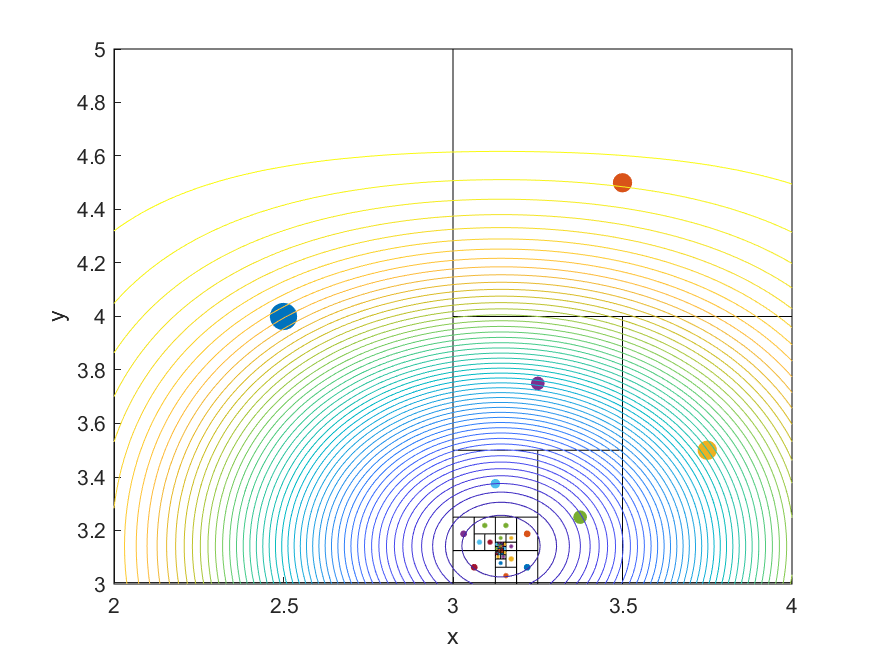
\includegraphics[width=0.9\textwidth]{Graphics/SimAnnealing_Easom_algo.png}
\caption{Работа метода отжига для функции Изома \eqref{Easom}} 
\end{figure}
\begin{figure}[H]
\centering
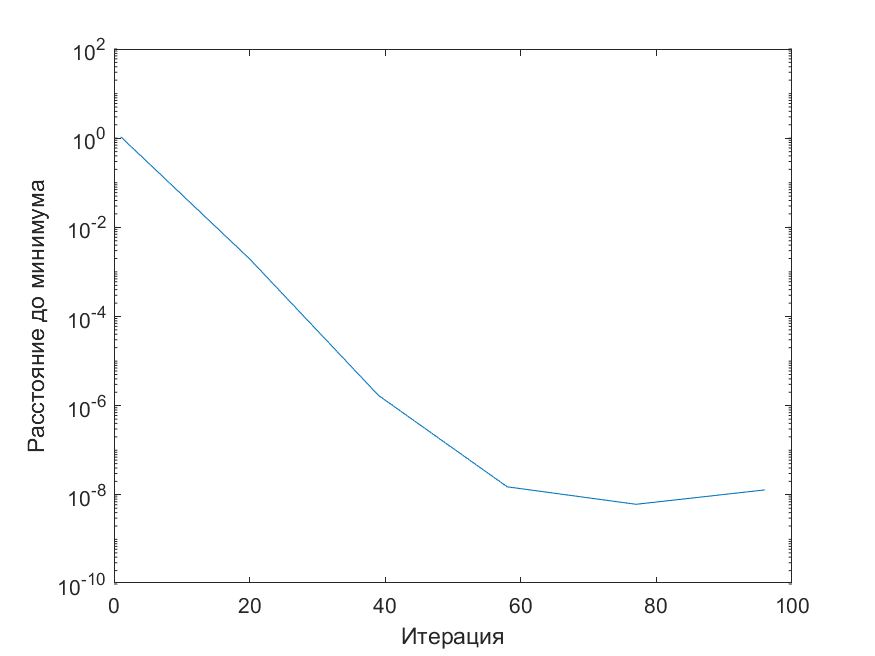
\includegraphics[width=0.9\textwidth]{Graphics/TrivialDivide_Easom_dist_to_min.png}
\caption{Расстояния до минимума простейшего алгоритма дробления\\ для функции Изома \eqref{Easom}} 
\end{figure}
\begin{figure}[H]
\centering
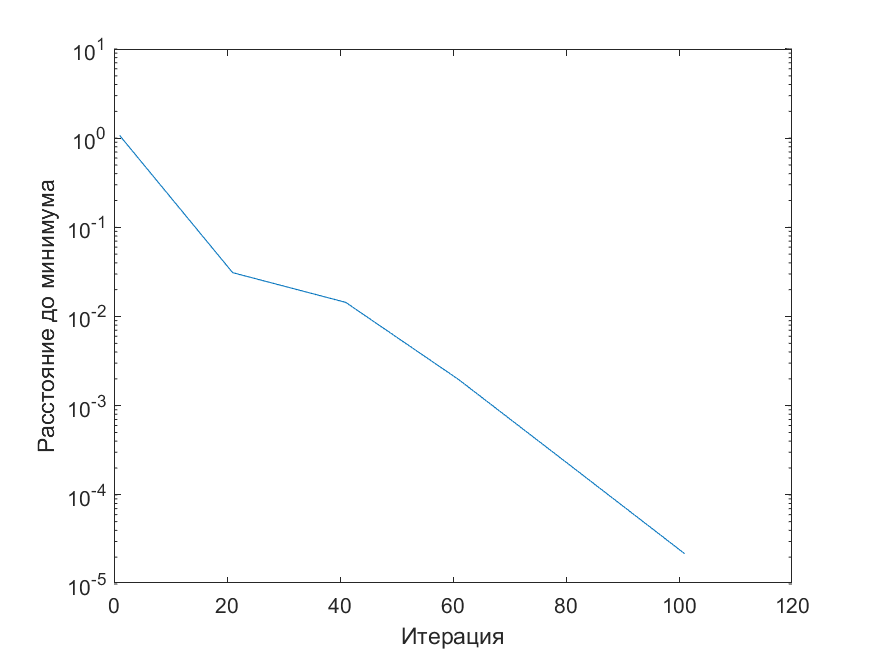
\includegraphics[width=0.9\textwidth]{Graphics/SimAnnealing_Easom_dist_to_min.png}
\caption{Расстояния до минимума метода отжига для функции Изома \eqref{Easom}} 
\end{figure}
\subsection{Функция <<шестигорбый верблюд>>}
Для функции <<шестигорбый верблюд>> положим $T_0=10, T_{\mathrm{fin}}=10^{-32}$ и $N_T=500$.\begin{figure}[H]
\centering
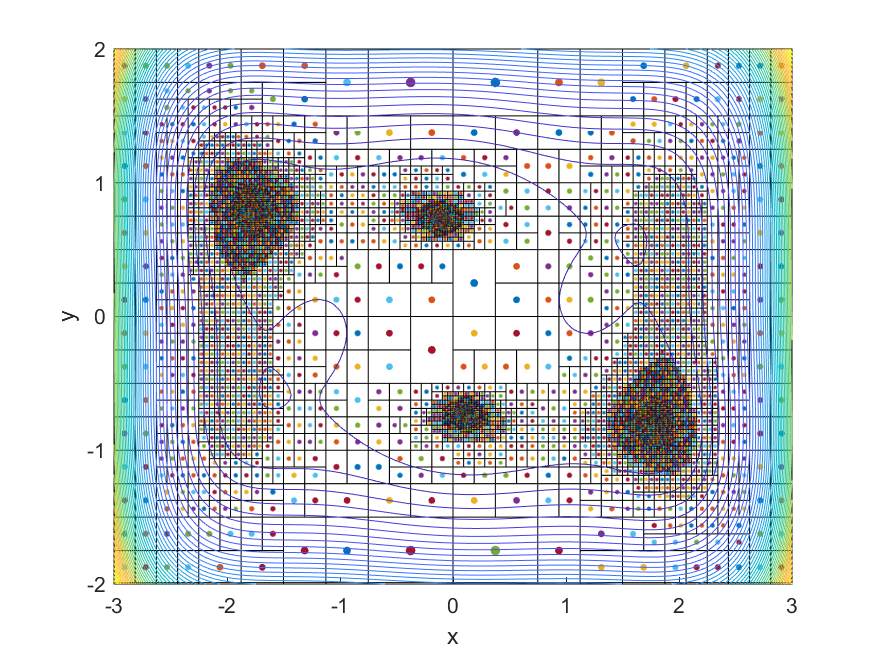
\includegraphics[width=0.9\textwidth]{Graphics/TrivialDivide_Camel_algo.png}
\caption{Работа простейшего алгоритма дробления \\ для функции <<шестигорбый верблюд>> \eqref{Easom}} 
\end{figure}
\begin{figure}[H]
\centering
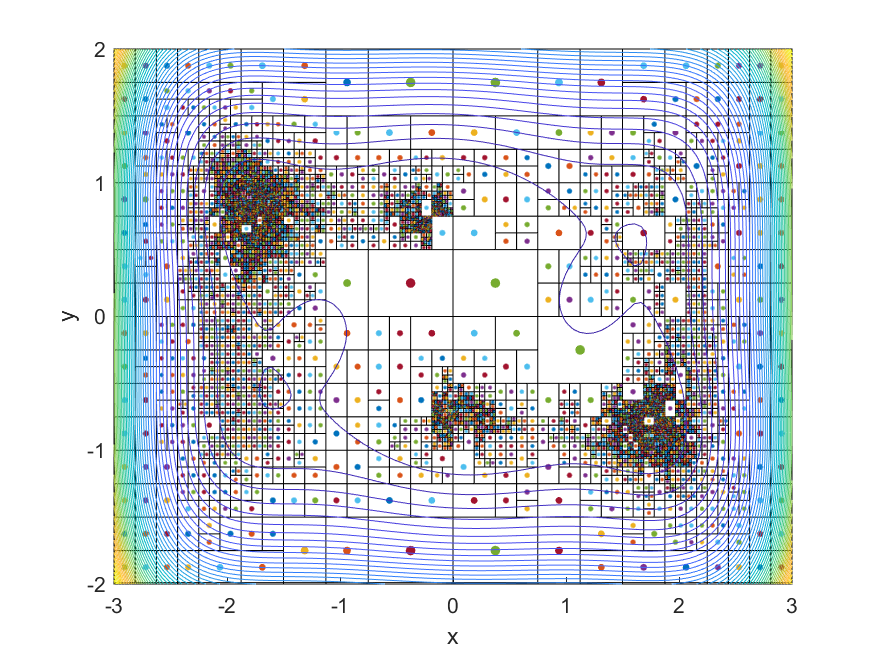
\includegraphics[width=0.9\textwidth]{Graphics/SimAnnealing_Camel_algo.png}
\caption{Работа метода отжига для функции <<шестигорбый верблюд>> \eqref{Easom}} 
\end{figure}
\begin{figure}[H]
\centering
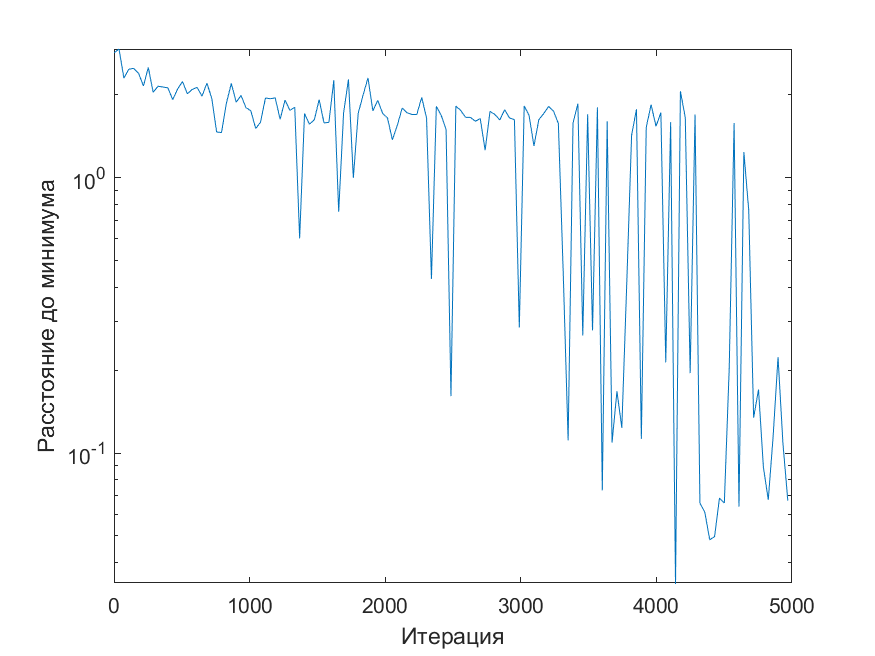
\includegraphics[width=0.9\textwidth]{Graphics/TrivialDivide_Camel_dist_to_min.png}
\caption{Расстояния до минимума простейшего алгоритма дробления\\ для функции <<шестигорбый верблюд>> \eqref{Easom}} 
\end{figure}
\begin{figure}[H]
\centering
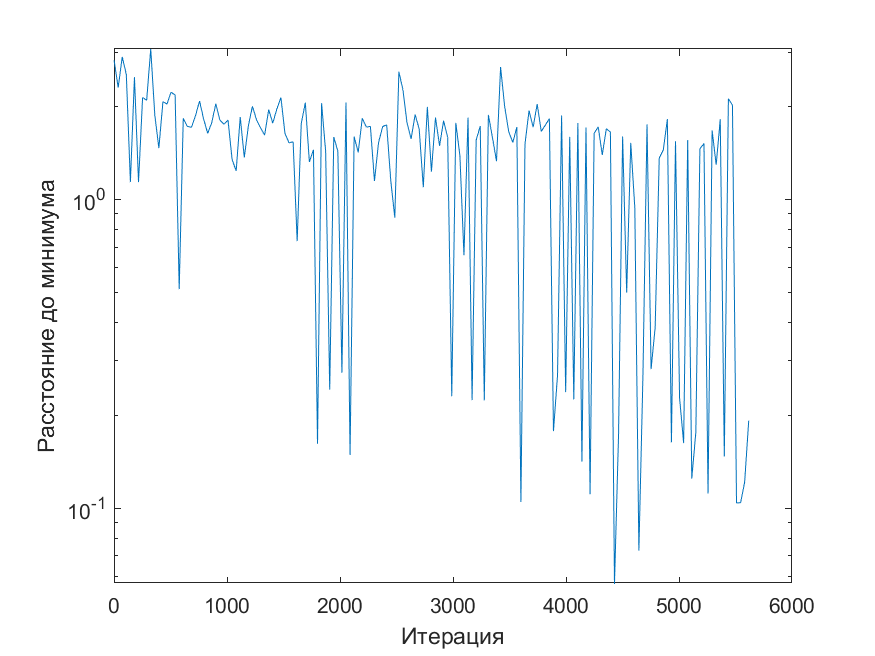
\includegraphics[width=0.9\textwidth]{Graphics/SimAnnealing_Camel_dist_to_min.png}
\caption{Расстояния до минимума метода отжига\\ для функции <<шестигорбый верблюд>> \eqref{Easom}} 
\end{figure}